\chapter{Results}

% PAST TENSE when describing work that I have done and each result section should refer to the aim that it is tackling

The aim of the methods described in this thesis is to develop and characterise tools to query the disequilibrium of sequence evolution. I present the test of existence and test of equivalence of process. Additionally, I present two new statistics for measuring the magnitude of disequilibrium. I evaluated these statistics on simulated data. Having selected statistical measures based of validation with data consistent with the null hypothesis, I applied my methods to naturally occurring cases of the alternate hypothesis aiming to validate whether they do, in fact, reflect an elevated level of disequilibrium. I report the application of my methods to two biological cases with striking prior evidence for recent perturbations affecting: an entire genome (loss of DNA methylation in \textit{D. melanogaster}); or, a small genomic segment (\textit{Fxy} in \textit{M. musculus}). I find that the methods are consistent with prior predictions made with knowledge of mechanism alone.  

\section{Developing and validating the methods}

A simple specification of a method is not enough, it was necessary to determine if it behaves in a way that matches up with the expectation when how the data is generated is known. Since I am interested in departures from being in equilibrium, that’s the condition set that I imposed in developing the methods. The process of validation began using the synthetic data sets in which the generating process is known to be in equilibrium. For some statistics, it was necessary to establish their properties on alignments that range in their evolutionary divergence, for this I used the observed Microbial data set.  

\subsubsection*{The best method of model fitting is without initialisation}

A necessary precursor to the application of any methods was to establish approximately optimal fits of the models. The initialisation experiment revealed that there are no intrinsic problems with the fitting process for GN or GNS. A fit was considered poor if the log-likelihood from the initialised method was higher than that of the uninitialised method. There were no occurrences of poor fits for any of the synthetic alignments. Initialised fits which were faster than the corresponding uninitialised fits were rare, occurring at a rate of about ~1\%. These results suggest that the best method of fitting for both models is without initialisation.

\subsubsection*{The LRT for Existence with parametric bootstrapping provided a robust estimation of significance}

To determine whether a given LRT statistic is significant requires establishing the appropriate null distribution. Statistical theory states that under certain conditions, the LRT statistic will be $\chi^2_{df}$ distributed with degrees freedom (df) equal to the difference in the number of free parameters between the models. In which case, one can obtain the $\hat p$-values for a given LRT statistic simply from the analytical distribution. The behaviour of the TOE with real finite data is unknown. When considering the use of mixed discrete- and continuous-time Markov process is a deviation from convention, it is especially important to establish whether the test statistic is consistent with theoretical expectations. 

The distribution is closer to but still not consistent with theoretical expectations for longer sequences, depicted in Figure \ref{fig:synthetic/lrt/197113-long_seq}. For alignments of length 300bp, shown in Figure \ref{fig:synthetic/lrt/197113-long_seq}a, the distribution of TOE statistic yields an excess of small p-values. Consequently, the data points of the Quantile-Quantile plot fall well below the diagonal line. Owing to increasing the power of the test, the distribution of p-values for longer alignments, illustrated in Figure \ref{fig:synthetic/lrt/197113-long_seq}b, is less skewed. Overall, the data points fall much closer to the diagonal line. The figure shows data generated from the same High JSD, High Entropy seed, however, the results for all seeds were very similar, see appendix Figure \ref{fig:synthetic/lrt/all-seeds}. 

\begin{figure}[htbp]
\centering
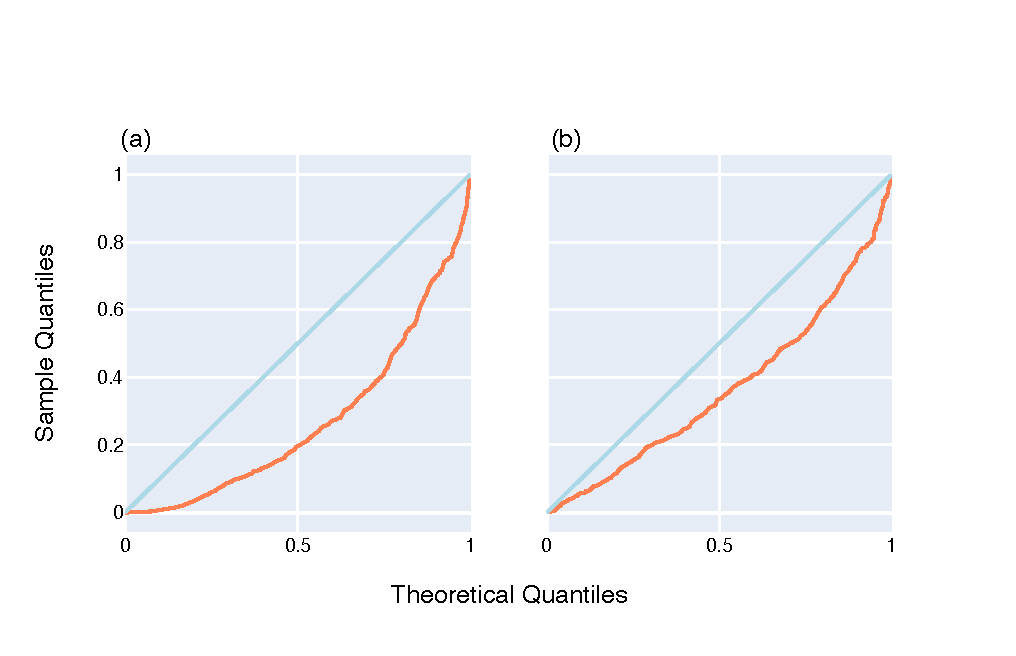
\includegraphics[width=\textwidth]{figures/plots/synthetic/lrt/197113_332182_17210-long_seq.pdf}
\caption[Increasing the length of the alignments gives a distribution of $\hat p-$ values closer, but not consistent with theoretical expectations]{\textbf{Increasing the length of the alignments gives a distribution of $\hat p-$ values closer, but not consistent with theoretical expectations.} The Quantile-Quantile (Q-Q) plots compare the $\hat p$-value distribution of the test for existence in stationary simulated data to the uniform distribution (pink line). Theoretical expectation is illustrated by the diagonal (blue line). Q-Q plot for \textbf{(a)} synthetic alignments of length $300$bp, \textbf{(b)}, synthetic alignments of length $30,000$bp. Each data set contains 1,000 synthetic stationary alignments. Both data sets shown are generated from the same high JSD, high entropy seed. The other seeds exhibited the same pattern, the result is shown in the appendix Figure \ref{fig:synthetic/lrt/all-seeds}.}
\label{fig:synthetic/lrt/197113-long_seq}
\end{figure}

The exploration with synthetic data clearly informs the application of my test. Firstly, the results of the initialisation experiment show there is no intrinsic fitting problems. As such, model fitting in all cases will be done without initialised parameter estimates. The results in Figure \ref{fig:synthetic/lrt/197113-long_seq} demonstrate that I cannot assume the TOE statistic to be $\chi^{2}$ distributed. As conventional asymptotic approximations to the TOE distribution are shown not to apply, significance levels will need to be assessed via a parametric bootstrap. 

\subsubsection*{A transformed $\nabla$ statistic exhibited robust behaviour under the null}

I present a novel statistic $\nabla$, which is a measure of the speed of convergence of the actual process to equilibrium. Consider a process operating on a single edge of a phylogenetic tree for a time interval of length $t$, for which the frequencies of nucleotides at the root is $\pi_0$ and the rate matrix on the edge is $Q$. The nucleotide distribution at $t$ is $\pi(t) = \pi_{0} \cdot e^{Qt}$. For a stationary process, this simplifies to $\pi(t) = \pi_{0}$. Under weak assumptions, a non-stationary process will converge to a stationary process, for which $\pi$ remains unchanged over time. Thus, I can describe the speed of this convergence with the rate of change of $\pi(t)$. In other words, the derivative of $\pi$ with respect to $t$,
\begin{equation}
\label{eq:dpi/dt}
\frac{\partial \pi}{\partial t}(t) = \pi_{0} \cdot Q \cdot e^{Qt}.
\end{equation}

To describe the magnitude of a vector in a single value, it is natural to take its length. Accordingly, the $\nabla$ statistic is defined as follows,
\begin{equation}
\label{eq:len-dpi/dt}
\nabla = ||\frac{\partial \pi}{\partial t}(t)|| =|| \pi_{0} \cdot Q \cdot e^{Qt}||.
\end{equation}
$\nabla$ is the magnitude of the rate of change of $\pi(t)$. For a stationary process, for which by definition $\pi$ does not change over time, $\nabla = 0$. For a non-stationary process, as the process approaches equilibrium, $\nabla$ will asymptote to $0$. For a given non-stationary process that converges monotonically to equilibrium, $\nabla$ must increase the further one moves from equilibrium. The algorithm used to calculate $\nabla$ is presented in Algorithm \ref{alg:convergence}.

\begin{algorithm}[ht!]
\caption[Algorithm]{Calculating $\nabla$}
\label{alg:convergence}
\begin{minted}{python}
def convergence(pi_0, Q, t):

    pi_deriv = dot(pi_0, dot(Q, expm(Q * t)))
    conv = norm(pi_deriv)

    return conv
\end{minted}
\end{algorithm}


The $\nabla$ statistic required a transformation to address bias introduced by shorter sequences. Presented in Figure \ref{fig:synthetic/d-conv-vs-conv/HighJSDHighEntropy}a are the distributions of $\hat \nabla$ in simulated data sets generated by the same stationary seed, but for alignments of length 300, 3,000, and 30,000. Figure \ref{fig:synthetic/d-conv-vs-conv/HighJSDHighEntropy}a shows that not only was there more variation in $\hat \nabla$ for the shorter alignments, but the location of the mean differed between lengths. The High JSD, High Entropy seed is shown in Figure \ref{fig:synthetic/d-conv-vs-conv/HighJSDHighEntropy}a, however, this result was the same for all seeds, included in the appendix (see Figure \ref{fig:synthetic/conv/all_seeds}). Empirical applications must compare statistics between sequences of different lengths, for which the $\nabla$ statistic required a transformation. 

\begin{figure}[htbp]
\centering
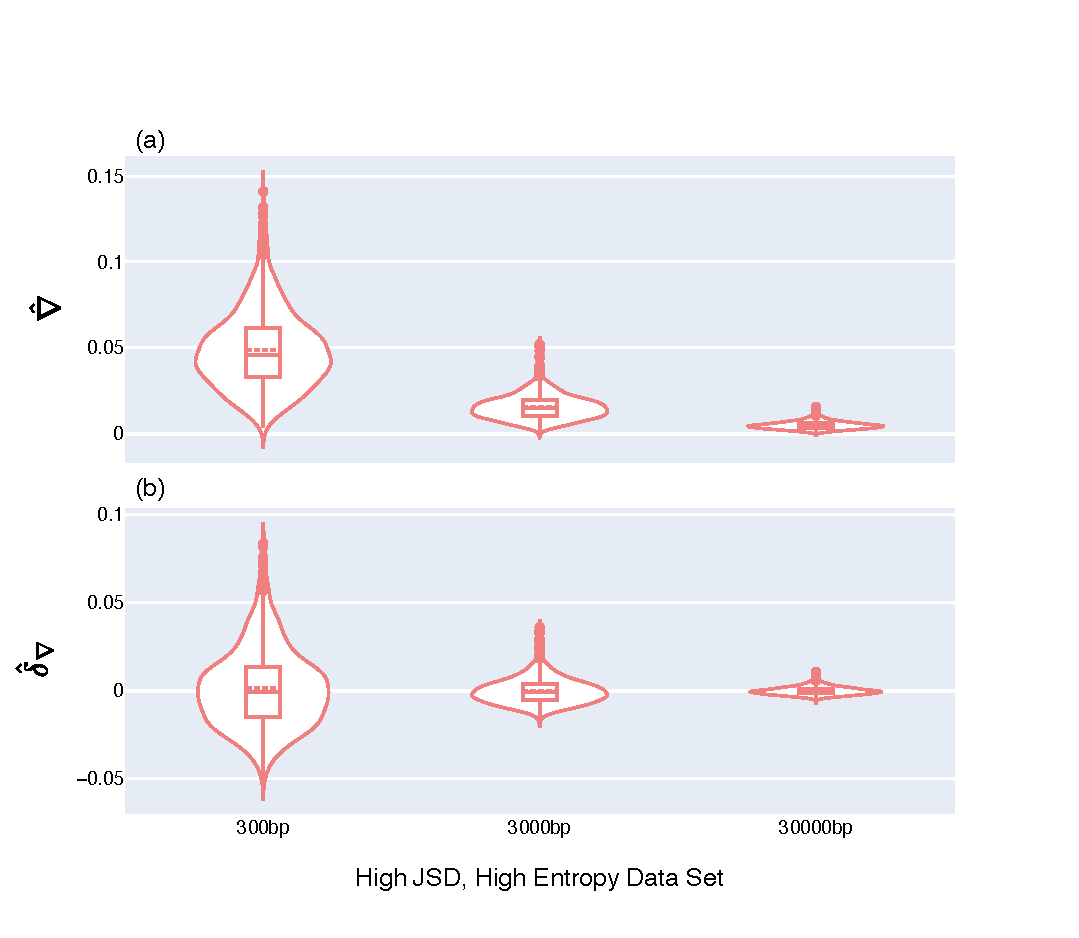
\includegraphics[width=\textwidth]{figures/plots/synthetic/d-conv-vs-conv/High JSD, High Entropy.pdf}
\caption{\textbf{The transformed statistic, $\delta_\nabla$, corrects for error introduced by the length of the alignment.} The violin plots show the distribution of $\hat \delta_\nabla$ for simulated data sets of alignment length 300, 3,000, and 30,000. \textbf{(a)} The original statistic, $\nabla$, had both a higher level of variation and a higher expected value in shorter sequences. \textbf{(b)} The transformed statistic $\delta_\nabla$ corrects for the location of the expected value only. The variation in shorter sequences remains, however, the mean for alignments of all lengths is centred on zero. Each data set contains 1,000 synthetic stationary alignments. The High JSD, High Entropy seed is shown, however, this result was the same for all seeds, included in the appendix (see Figure \ref{fig:synthetic/conv/all_seeds}). }
\label{fig:synthetic/d-conv-vs-conv/HighJSDHighEntropy}
\end{figure}

The selected transformation, denoted $\delta_\nabla$, adjusted for location only, ensuring the expected value was zero when the null was true. For a given alignment, $\hat \delta_\nabla$ is the difference between the observed $\hat \nabla$ and the mean  $\hat \nabla$ of synthetic alignments generated under the null, $\delta_\nabla =  \nabla - \mu_{\nabla{null}}.$ Presented in Figure \ref{fig:synthetic/d-conv-vs-conv/HighJSDHighEntropy}b are the distributions of $\hat \delta_\nabla$ in simulated data sets again generated by the High JSD, High Entropy seed for alignments of length 300, 3,000, and 30,000. \ref{fig:synthetic/d-conv-vs-conv/HighJSDHighEntropy}b shows that the expected value of the transformed $\delta_\nabla$ statistic is close to zero when the null is true. Although there is more variation in the shorter sequences, this simple method of transformation was chosen because the statistic retains the same units as the untransformed statistic. 
% Normality?

The $\delta_\nabla$ statistic increases with a known marker of historic disequilibrium. As described in the methods, JSD is an information theoretic measure of the difference between probability distributions. Therefore, the JSD between two edges of a tree is an indication of the level of historic disequilibrium in one or more of the lineages. The $\delta_\nabla$ statistic has a strong positive relationship with the JSD between ingroup edges for taxa from the microbial data set, illustrated in Figure \ref{fig:microbial/d-conv/JSD}. This relationship is very encouraging as it supports that $\delta_\nabla$ is in fact measuring what it is intended to measure, mutation disequilibrium. 

\begin{figure}[htbp]
\centering
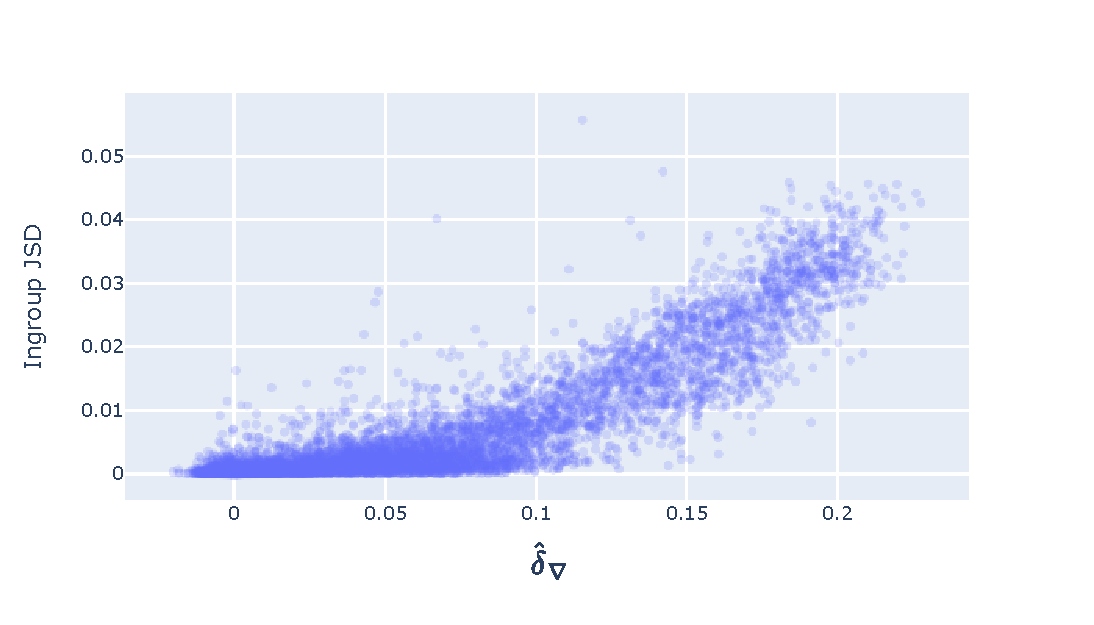
\includegraphics[width=\textwidth]{figures/plots/microbial/d-conv-JSD.pdf}
\caption{\textbf{The $\hat\delta_\nabla$ statistic increased with a marker of historic disequilibrium.} The scatter plots shows magnitude of disequilibrium measure by $\hat\delta_\nabla$ and the JSD between ingroup taxa for the observed Microbial data set. The Microbial data set comprises 9702 alignments where the level of disequilibrium is expected to vary.}
\label{fig:microbial/d-conv/JSD}
\end{figure}

\subsubsection*{The $T_{50}$ statistic exhibited paradoxical propertied that prevented interpretation}

A seemingly natural way to describe disequilibrium in a system is by its proximity to equilibrium. As previously stated, for a process in disequilibrium, as time goes to infinity, its nucleotide distribution will converge to $\pi_\infty$, its equilibrium distribution. This can be expressed mathematically as 
$$\pi_\infty = \lim_{t \to \infty}\pi \cdot e^{\mathbf{Q}t}.$$ 
This property manifests in other situations, for example, the decay of a radioactive element. In those fields the problem of quantification is solved by expressing in terms of an arbitrarily chosen metric, half-life, the time taken until half of the element's original mass is left. $T_{50}$ is defined equivalently. ${T_{50}}$ is a measure of the distance to halfway to $\pi_\infty$, measured in terms of the expected number of substitutions. The algorithm used to calculate $T_{50}$ is presented in Algorithm \ref{alg:t50}.

\begin{algorithm}[ht!]
\caption[Algorithm]{Calculating $T_{50}$}
\label{alg:t50}
\begin{minted}{python}
class T50:
    def __init__(self, Q, pi_0, func=jsm):
        """
        func
            a callback function that takes two probability vectors
            and returns a "distance". Defaults to Jensen-Shannon metric.
        """
        self.Q = Q
        self.pi_0 = pi_0
        self.pi_inf = self.get_stat_pi()
        self.dist_halfway = func(self.pi_0, self.pi_inf) / 2
        self.tau = 1
        self.dist_func = func

    def get_stat_pi(self):
        return get_stat_pi_via_brute(expm(self.Q), self.pi_0)

    def estimate_t50(self):
        ens_curr = expected_number_subs(self.pi_0, self.Q, 1)
        self.tau = minimise(
            self,
            xinit=self.tau,
            bounds=([1], [1e10]),
            local=True,
            show_progress=False,
            tolerance=1e-8,
        )
        ens_50 = expected_number_subs(self.pi_0, self.Q, self.tau)
        return ens_50 - ens_curr

    def distance_from_pi_zero(self, pi):
        return self.dist_func(self.pi_0, pi)

    def __call__(self, tau):
        pi_tau = dot(self.pi_0, expm(self.Q * tau))
        dist1 = self.dist_func(self.pi_0, pi_tau)
        dist2 = self.dist_func(pi_tau, self.pi_inf)
        return abs(dist1 - dist2) ** 2
\end{minted}
\end{algorithm}


The algorithmic routines used in calculating the $T_{50}$ statistic were vulnerable to machine precision errors. The testing of $T_{50}$ illustrated a simple error that can arise from calculations using \gls{floating point arithmetic}. Consider the following equation, $1e16 + 1.0 - 1e16$. This should equal $1$, however, using a computer, it will evaluate to $0$. Such is a simple example of how the representation of numbers in computers can propagate errors in calculations. One test case for $T_{50}$ was, given model parameters generated by GTR, where by definition the nucleotide distribution is stationary, the returned value should be $0$. Interestingly, this test was failing. Debugging revealed that the failure was due to machine precision errors. Following this discovery, code for $T_{50}$ was changed to use accurate algorithms for floating point sums and dot products \citep{accupy}. These algorithms avoid possible imprecision by tracking multiple intermediate partial sums, a routine that does come with a modest speed loss \citep{Shewchuk1997AdaptivePredicates, Ogita2005AccurateProduct}. 

Even using the most precise algorithms, the estimation of $T_{50}$ was extremely vulnerable to sampling error. The simulated data was generated to be stationary, meaning the expectation was for $T_{50}$ to be zero, of course, this is never quite the case because of sampling error. The error was unmistakable in data generated by the High JSD, Low Entropy seed, shown in Figure \ref{fig:T50-short_long}, where the outlying values for shorter alignments completely obscure the shape of the distributions. Although most pronounced in the seed shown, higher sampling error in the shorter sequences was a feature of all seeds, shown in the appendix (see fig. (ref)). 

\begin{figure}[!ht]
\centering
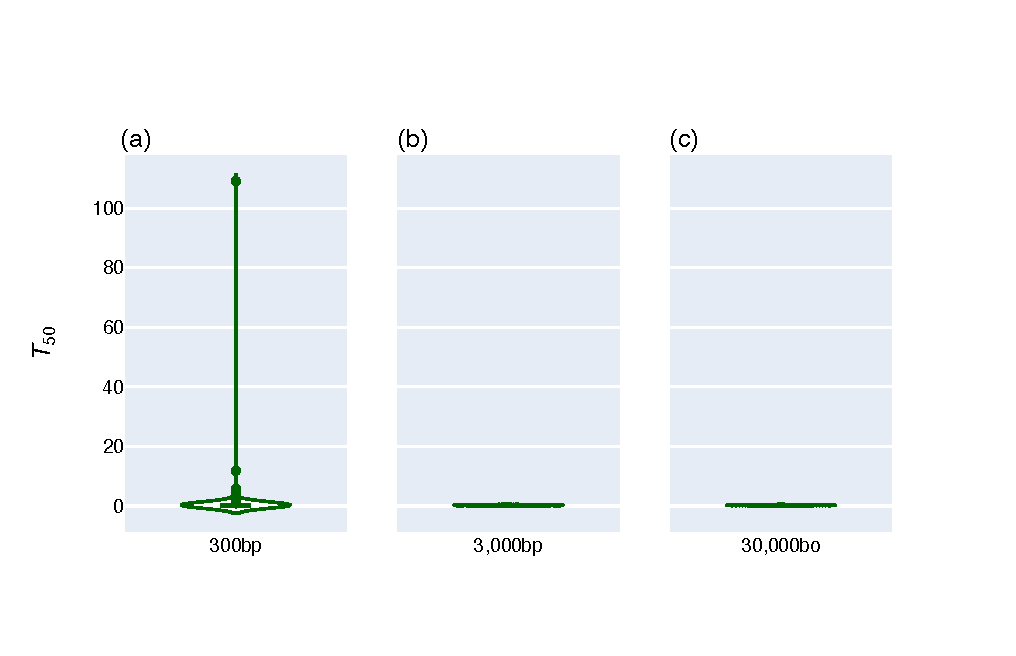
\includegraphics[width=\textwidth]{figures/plots/synthetic/T50/HighJSDLowEntropy-seq_len.pdf}\caption{\textbf{Long Alignments have less sampling error}}
\label{fig:T50-short_long}
\end{figure}

$T_{50}$ estimated under the null was not robust to features of the data. In the simulated stationary data, $T_{50}$ appeared to have a bias towards being highest in the low JSD seeds. The median $\hat T_{50}$ for all simulated data sets is shown in Table \ref{t50_means}. In all but one case, when grouped by length and entropy, the median $\hat T_{50}$ for low JSD $>$ the median $\hat T_{50}$ for high JSD. Recall that JSD is used throughout as a marker of historic disequilibrium. Even though in the simulated data the foreground edge changed to be stationary, it was expected that in the high JSD data sets there would be more disequilibrium in the background edges. It is thus unexpected both that there is a pattern, and that the pattern reflects higher disequilibrium in the low JSD data. This was unexpected and conflicted with the understanding of both $T_{50}$ and JSD.  As a consequence, I did not continue to use $T_{50}$ and you will not see it in further results.

\begin{table}[htbp]
\begin{tabularx}{\textwidth}{ 
  | >{\centering\arraybackslash}X
  | >{\centering\arraybackslash}X 
  | >{\centering\arraybackslash}X 
  | >{\centering\arraybackslash}X  
  | >{\centering\arraybackslash}X | }
\hline  
\textbf{Alignment Length} &\textbf{ High JSD, Low Entropy} & \textbf{ Low JSD, Low Entropy} & \textbf{High JSD, High Entropy} & \textbf{Low JSD, High Entropy} \\
\hline 
    \textbf{300bp} & 0.3184 & 0.3363 & 0.3497 & 0.4576 \\
    \textbf{3,000bp} & 0.2663 & 0.2563 & 0.3096 & 0.3990 \\
   \textbf{30,000bp} & 0.2514 & 0.2778 & .3107 & 0.3911 \\ 
\hline 
\end{tabularx}
\caption{\textbf{Median $\hat T_{50}$ for simulated stationary data sets.} In all but one case, when grouped by length and entropy, the median $\hat T_{50}$ for low JSD exceeded the median $\hat T_{50}$ for high JSD. Each data set contained 1,000 synthetic stationary alignments.}
\label{t50_means}

\end{table}


\subsubsection*{Both tests of equivalence of process were consistent with asymptotic approximations}

 As described in the methods, the EOP tests are hypothesis tests for whether the process is shown to be different. This can be applied to two comparison, adjacent and temporal. Adjacent is the test of equivalence between neighbouring alignments of the same edge and temporal is the test between one-to-one orthologs. Both tests are a comparison of likelihoods between fitting both alignments with one $\mathrm{Q}$ (null), or fitting a separate $\mathrm{Q}$ per alignment (alternate). Significance is assessed with a likelihood ratio, which again, it is necessary to determine whether asymptotic approximations apply. 

Applying both tests to their respective null distributions indicated that they are both consistent with theoretical expectations, presented in Figure \ref{fig:synthetic/adj-temp_eop/HighJSDHighEntropy}. This is illustrated by Quantile-Quantile plots comparing the distribution of p-values to the uniform distribution for the temporal test (fig. \ref{fig:synthetic/adj-temp_eop/HighJSDHighEntropy}a) and the adjacent test (fig. \ref{fig:synthetic/adj-temp_eop/HighJSDHighEntropy}b). The orange line falls very close to the diagonal, demonstrating that the distribution of $\hat p-$values is almost indistinguishable from the uniform distribution.  This result identifies that in application of this test, it is suitable to assume the statistic is $\chi^2_{df}$ distributed and in turn, obtain the $\hat p-$value from analytical distribution. Alignments of length 300 generated by the High JSD, High Entropy seed are shown, however, this result was the same for all seeds and all lengths, included in the appendix (see Fig. \ref{fig:synthetic/adj_eop/all_seeds} and \ref{fig:synthetic/temp_eop/all_seeds}).

\begin{figure}[htbp]
\centering
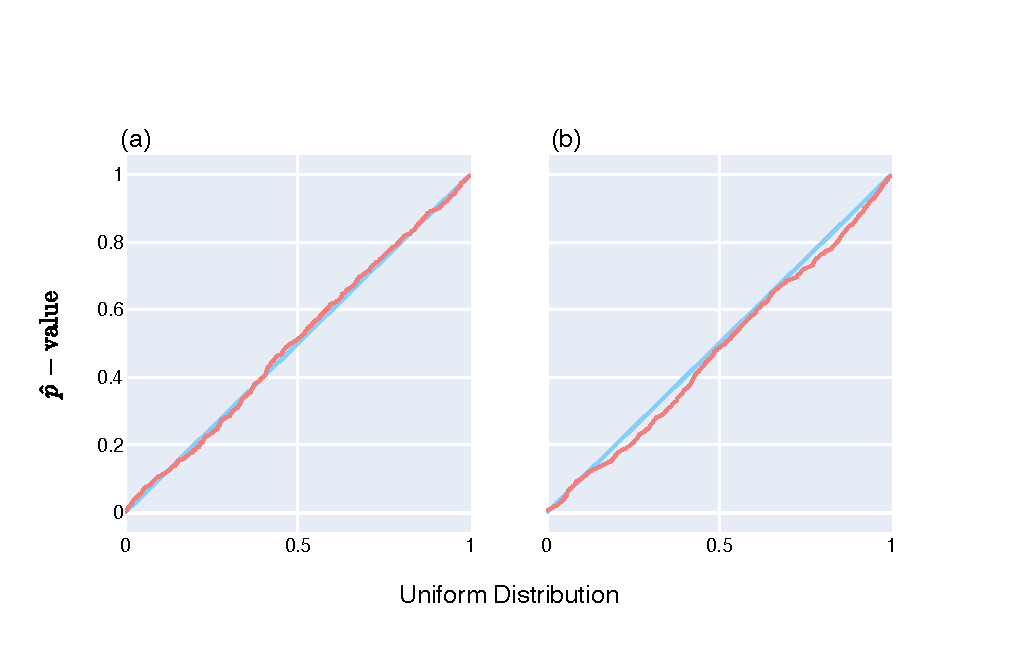
\includegraphics[width=\textwidth]{figures/plots/synthetic/adj-temp_eop/High JSD, High Entropy.pdf}
\caption{\textbf{Both equivalence of process tests were consistent with theoretical approximations.} The Quantile-Quantile plots compare the distribution of $\hat p-$values to the uniform distribution. As the data points (shown as the orange line) fall very close to the diagonal, this demonstrates that the distribution of $\hat p-$values is almost indistinguishable from the uniform distribution. (a) $\hat p-$values from temporal equivalence of process, (b) $\hat p-$values from adjacent equivalence of process. This result is shown for alignments of length 300 generated by the High JSD, High Entropy seed, however, the result was the same for all seeds and all lengths, shown in the appendix, see figure \ref{fig:synthetic/adj_eop/all_seeds} and \ref{fig:synthetic/temp_eop/all_seeds}.}
\label{fig:synthetic/adj-temp_eop/HighJSDHighEntropy}
\end{figure}

\section{Testing the known}

Having lost major components of the DNA methylation process that remain in its sister taxa, the \textit{D. melanogaster} genome is a very useful natural experiment. DNA methylation is a well known mutagenic force. Consequently, the lack thereof in
\textit{D. melanogaster} led to the strong prediction that the \textit{D. melanogaster} genome would exhibit globally high levels of mutation disequilibrium. \textit{D. simulans} still methylates its DNA, which provided a necessary point of comparison. I performed two separate analyses, each with either \textit{D. melanogaster} or \textit{D. simulans} as the foreground, and another close taxa that retains methylation, \textit{D. yakubra}, as the outgroup. The analyses were performed on the same alignments of the Drosophila data set, which contains third codon positions from orthologous CDS alignments. The aim was to determine whether the developed methods would reflect the expected form of mutation disequilibrium. The expectations were that the \textit{D. melanogaster} genome would exhibit higher levels of both existence and magnitude of mutation disequilibrium than \textit{D. simulans} and that this would be a genome wide relationship. The relative levels of purifying natural selection operating on the chromosomes allows for predictions of the magnitude of mutation disequilibrium in the chromosomes. Thus, a further expectation was that the X chromosome would exhibit a higher magnitude of mutation disequilibrium relative to the autosomes. 

\subsubsection*{The entire \textit{D. melanogaster} genome is systematically elevated in both the existence and magnitude of mutation disequilibrium compared to its sister taxa, \textit{D. simulans}}

There is a striking elevation of the existence of mutation disequilibrium in the \textit{D. melanogaster} genome when compared to that of \textit{D. simulans}, shown in Figure \ref{fig:drosophila_lrt_qq}. Each subplot in Figure \ref{fig:drosophila_lrt_qq} shows for the observed data, as well as simulated +ve and -ve controls, the distribution of $\hat p-$ values from the TOE compared to the uniform distribution. The controls are two synthetic cases of ground truth no disequilibrium (-ve), and ground truth there is disequilibrium (+ve), used to determine how reliable the estimates are. Each data point from the +ve and -ve controls was simulated using model parameters from a corresponding observed alignment.  The observed data points of \textit{D. melanogaster}, shown in Figure \ref{fig:drosophila_lrt_qq}b, fall substantially further from the -ve control than that of \textit{D. simulans}, shown in \ref{fig:drosophila_lrt_qq}a. This indicates that, as specified by the TOE, a much larger proportion of the \textit{D. melanogaster} genome is in mutation disequilibrium than \textit{D. simulans}. The specific proportion of each genome, requires correcting for multiple tests of the same hypothesis. 

\begin{figure}[h]
\centering
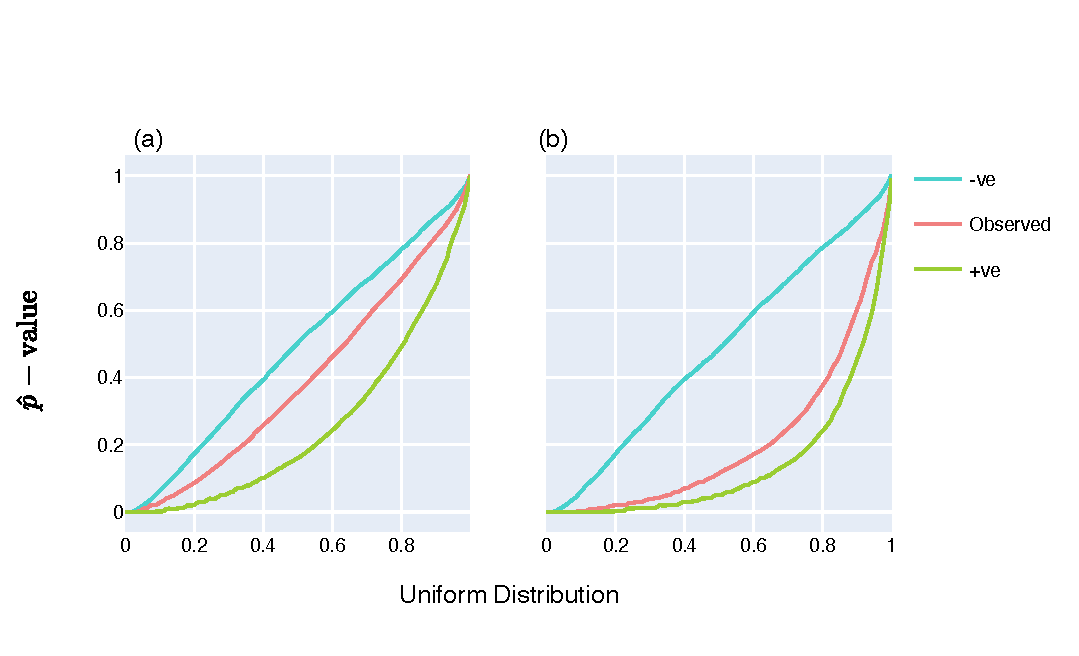
\includegraphics[width=	\textwidth]{figures/plots/drosophila/LRT-QQ.pdf}
\caption{}
\label{fig:drosophila_lrt_qq}
\end{figure}


The resolution of $\hat p-$ values is too low for conventional methods of multiple test corrections. The simulation results revealed that under the theoretical distribution the TOE  $\hat p-$ values are not uniformly distributed. As a result, they are unsuitable for assessing significance. A method for assessing significance, in this case, is with a parametric bootstrap. The compute time for a bootstrap with a single replicate is ${\sim} 6$ seconds. For the \textit{Drosophila} data sets there are ${\sim} 4,500$ alignments. In order to satisfy the Bonferroni correction for $4,500$ alignments you would need to, with some level of precision, be able to estimate $p$ values below the altered significance threshold, $0.05/4,500 = 1.1{\times}10^{-5}$. For it to be possible to reject the null requires generating greater than $1/1.1{\times}10^{-5}$ replicates per alignment. This would take $9,009$ hours per alignment, of which considering both taxa, there are $>9,000$. This is a prohibitive level of computation that is both impractical, and unnecessary. 

I have established an alternate strategy that takes advantage of the shape of the distribution. The challenge of correcting for multiple tests is pronounced in the space of genomics, for which \cite{Storey2003StatisticalStudies} introduced a formal procedure for estimating the false discovery rate. In their case, they produce an alternate statistic to be interpreted for an individual result, which isn't applicable here due to the low resolution of $p-$values. However, their procedure included an estimation of the fraction of an analysis which is consistent with the null hypothesis. This method takes advantage of how the $p-$values of data that is consistent with the null will be uniformly distributed, illustrated in Figure 1 of \citep{Storey2003StatisticalStudies}. Fitting a cubic spline to determine the inflection point, one can estimate the proportion of a given distribution that is uniform consistent with the null hypothesis, denoted here as $f$. Of interest to this analysis is $1 - f$, the proportion that is not consistent with the null hypothesis. The code to produce $f$ is included in the \href{https://github.com/StoreyLab/qvalue}{qvalue} R package \citep{Storey2004StrongApproach}.

A significantly higher proportion of the \textit{D. melanogaster} genome was estimated to be in mutation disequilibrium compared to \textit{D. simulans}. The estimated proportion ($1 - f$) of the \textit{D. melanogaster} genome which is in mutation disequilibrium was 90\% compared to 50\% of the \textit{D. simulans} genome. Such a substantial difference is a compelling result. Where there is strong evidence of the recent evolution of mutation, \textit{D. melanogaster}, the vast majority of genes are in mutation disequilibrium. In a closely related species where the state of mutation has not so drastically changed, \textit{D. simulans}, only half of the genes are in mutation disequilibrium. This result supports the prediction that the existence of mutation disequilibrium would be elevated in \textit{D. melanogaster} relative to its sister taxa.

The magnitude of mutation disequilibrium, as measured by the $\delta_\nabla$  statistic, is also higher in \textit{D. melanogaster}. Figure \ref{fig:drosophila_d-conv-diff} shows a direct comparison allowed by the paired nature of the data sets. Each data point in Figure \ref{fig:drosophila_d-conv-diff} is the difference between $\hat \delta_\nabla$ for a \textit{D. melanogaster} gene and its ortholog in \textit{D. simulans}. These are genes with essentially the same function, but evolving under presumably different mutagenic environments. The distribution in Figure \ref{fig:drosophila_d-conv-diff} is right shifted, showing that most genes have a higher $\delta_\nabla$ estimate in \textit{D. melanogaster}. This result supports the prediction that the magnitude of mutation disequilibrium would be elevated in \textit{D. melanogaster} relative to its sister taxa. 

\begin{figure}[h]
\centering
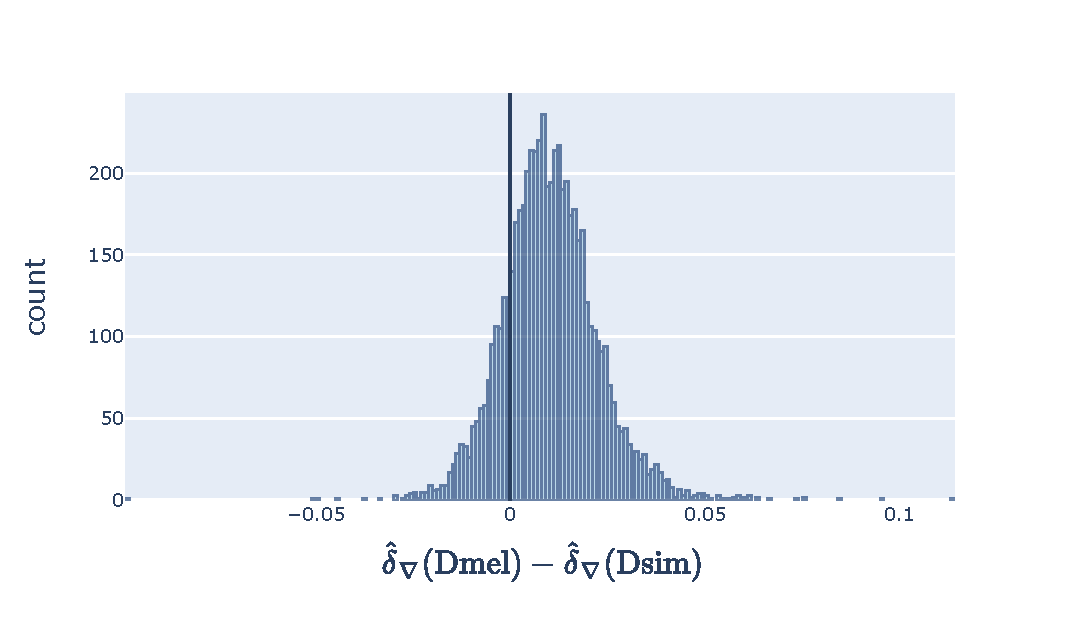
\includegraphics[width=	\textwidth]{figures/plots/drosophila/d-conv-diff.pdf}
\caption{\textbf{The magnitude of mutation disequilibrium is higher in \textit{D. melanogaster} genes.} }
\label{fig:drosophila_d-conv-diff}
\end{figure}


The pattern of elevated mutation disequilibrium is systematic across the \textit{D. melanogaster} genome. The mean $\hat \delta_\nabla$ for a chromosome is shown with a horizontal line in Figure \ref{fig:drosophila_d-conv_manhattan}, where for all chromosomes analysed, \textit{D. melanogaster} clearly exceeds \textit{D. simulans}. In fact, comparatively, the \textit{D. simulans} genome appears to be centred very close to zero. The consistency of elevation throughout the genome is in accordance with prior predictions.

Strong purifying selection appears to impedes the rate of convergence of the X chromosome. Considering that the X chromosome has fewer data points, it is evident in Figure \ref{fig:drosophila_d-conv-diff} that the \textit{D. melanogaster} X has an larger proportion of high $\hat \delta_\nabla$ than all other chromosomes shown. The median $\hat \delta_\nabla$ for chromosomes 2, 3 and X in \textit{D. melanogaster} is $0.0132$, $0.0131$ and $0.0177$ respectively. The median $\hat \delta_\nabla$ for chromosomes 2, 3 and X in \textit{D. simulans} is $0.0031$, $0.0031$ and $0.0040$ respectively. For both species the X chromosome clearly has a higher median $\hat \delta_\nabla$ than the autosomes, consistent with a slower rate of convergence and thus a higher magnitude of disequilibrium for sequence acted upon by purifying selection. 

\begin{figure}[htbp]
\centering
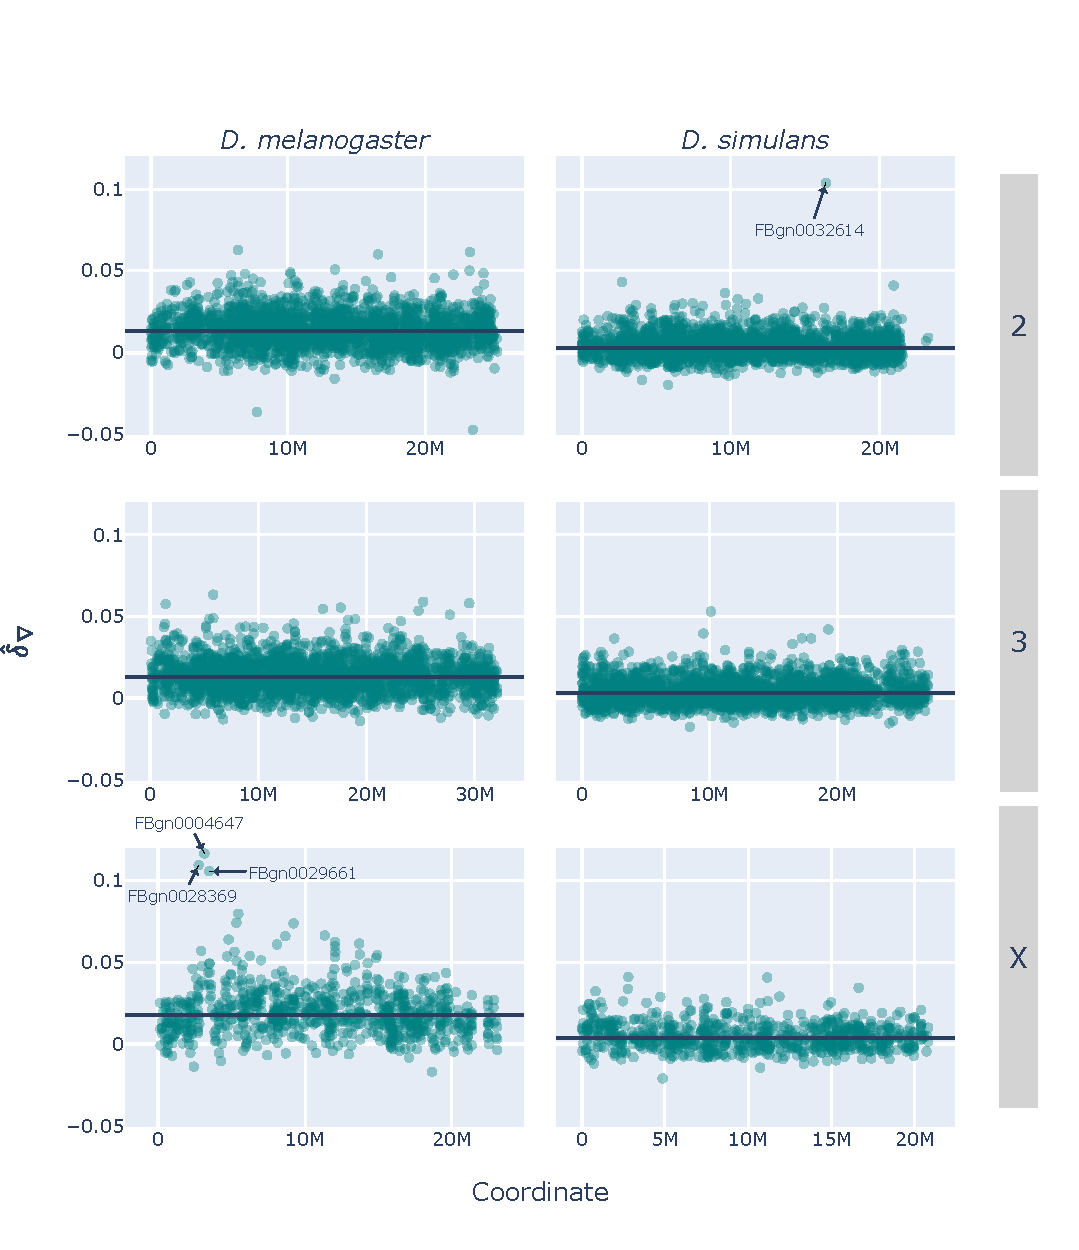
\includegraphics[width=\textwidth]{figures/plots/drosophila/d-conv_manhatten.pdf}
\caption{\textbf{The pattern of elevated mutation disequilibrium in \textit{D. melanogaster} compared to \textit{D. simulans} is systematic across the genome}. Manhattan plots the position of a gene in a chromosome and the $\hat\delta_\nabla$ for the CDS sequence of that gene. The CDS sequence is third codon position only. The median $\hat\delta_\nabla$ is indicated for a chromosome with a horizontal line. The number of genes included in the plots of chromosome 2, 3, and X of \textit{D. melanogaster} is 2373, 2624 and 818 respectively. For chromosome 2, 3, and X of \textit{D. simulans}, the number of genes is 2388, 2623 and 800 respectively.}
\label{fig:drosophila_d-conv_manhattan}
\end{figure}


Equivalence of process between Dm and Ds orthologs

\begin{figure}[ht!]
\centering
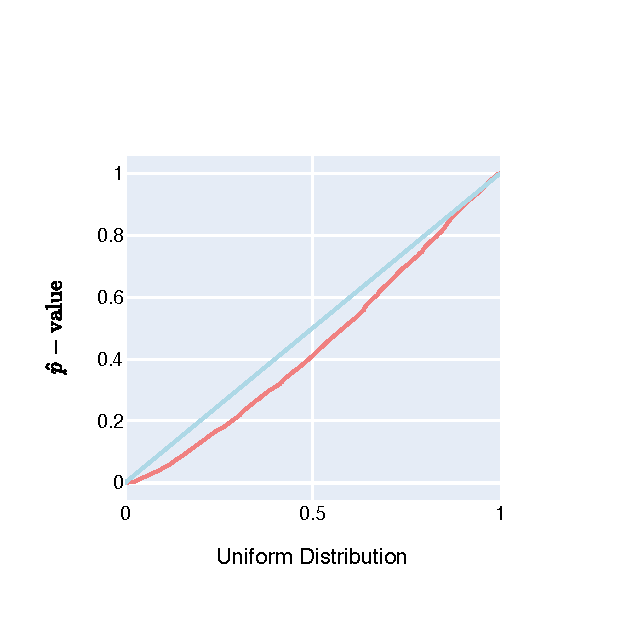
\includegraphics[width=0.6\textwidth]{figures/plots/drosophila/temp-EOP-QQ.pdf}
\caption[The mutagenic process was not distinguishable between \textit{D. melanogaster} and \textit{D. simulans}]{\textbf{The mutagenic process was not distinguishable between \textit{D. melanogaster} and \textit{D. simulans}.} The Quantile-Quantile plots compare the distribution of the temporal EOP between genes in \textit{D. melanogaster} and their ortholog in \textit{D. simulans} to  to the uniform distribution. The data points fall close to the diagonal indicating that the distribution is almost identical to what we would expect if the null was true. The plot shows 5,942 third codon position CDS alignments from \textit{D. melanogaster}, \textit{D. simulans} and \textit{D. yakubra}. }
\label{fig:drosophila:temp-EOP-qq}
\end{figure}



Link back to the aim and whether the result show what I aimed to show. 

\section{Testing the conjectured}

Recombination and its association with GC-biased gene conversion has been proposed to be a major force in the formation of isochores \citep{Montoya-Burgos2003RecombinationGenomes}. The translocation of \textit{Fxy} in \textit{M. musculus} such that half of the gene now resides in the only recombining part of the X chromosome is a unique natural experiment from which that conjecture may be corroborated. This perturbation is predicted to have led to elevated disequilibrium in the region that has moved into the PAR, relative to the component of the gene that remains in the uniquely X region. To test this prediction I used alignments of \textit{Fxy} in \textit{M. musculus} with orthologs from \textit{M. spretus} and \textit{R. norvegicus}. For all model fitting, \textit{M. musculus} was the foreground edge. I analysed the first six introns of Fxy, of which in \textit{M. musculus} the $5'$ end (exons 1-3) is X-specific, and the $3'$ end (exons 4-6) is located in the PAR. The boundary of the PAR is found in the third intron \citep{Palmer1997AMice}. The evolutionary history of \textit{Fxy} in rodents alongside the structure of \textit{Fxy} in \textit{M. musculus} is shown in Figure \ref{fig:Fxy}. 

I aimed to determine whether the current understanding of how this translocation may affect the divergence process would be reflected by the methods. Because the entire gene had been translocated, I expected the whole gene to be in mutation disequilibrium. Considering the distinct mutagenic properties of the PAR, I aimed to see whether by using the statistic of magnitude, $\delta_\nabla$, I could detect elevated levels of disequilibrium in the PAR-located half. A specific location of the boundary is not provided, therefore, I aimed to see whether the magnitude of mutation disequilibrium locally within intron 3 would illustrate where the boundary is located. 

\begin{figure}[htbp]
\centering
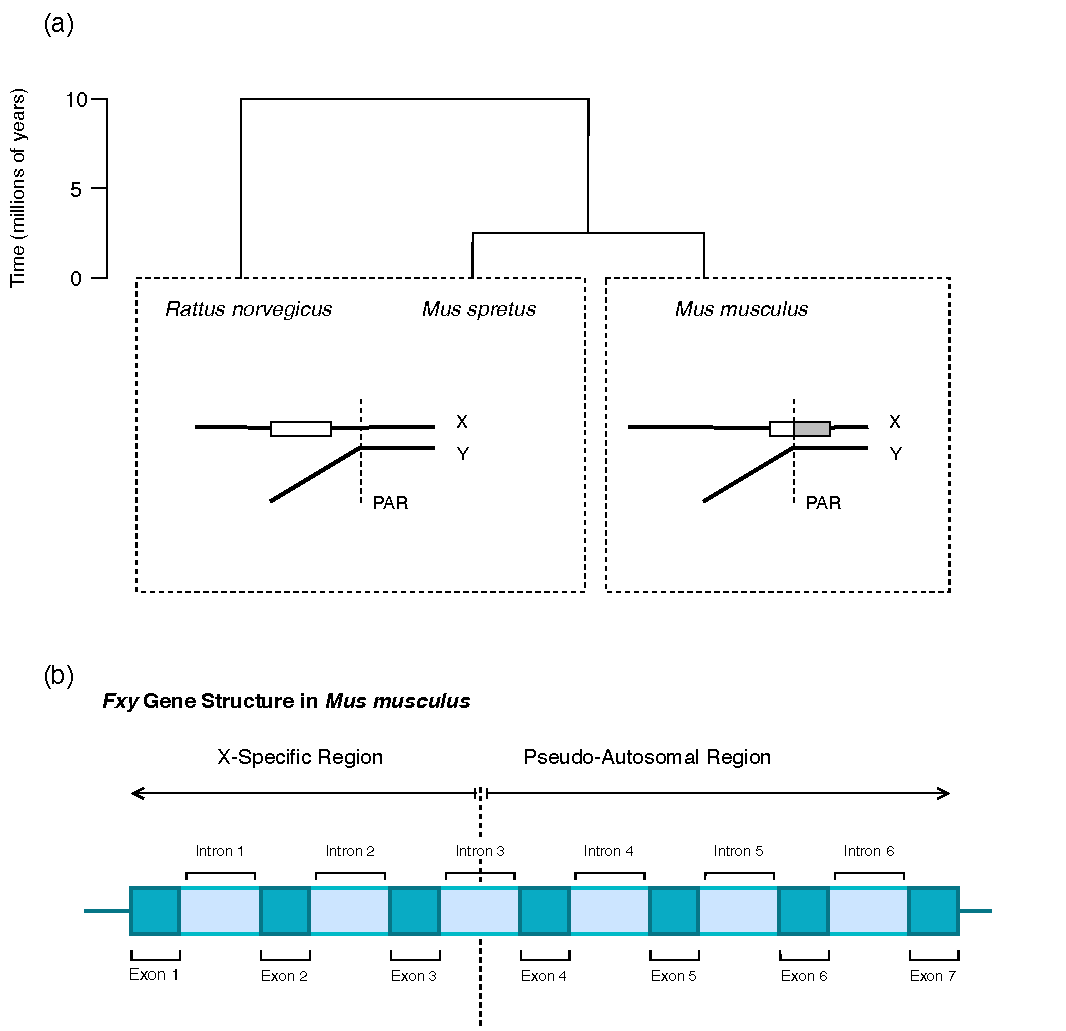
\includegraphics[width=\textwidth]{figures/diagrams/Fxy.pdf}
\caption[Evolutionary History of \textit{Fxy} in Rodents]{\textbf{Evolutionary History of \textit{Fxy} in Rodents}. \textbf{(a)} The \textit{Fxy} gene in \textit{M. musculus} was translocated from a X-specific position to a new position in which it overlaps with the PAR. The overlap in \textit{M. musculus} is shown as the shaded region of the gene, shown as a box. The divergence timescale is indicated in millions of years. In rodents and other mammals \textit{Fxy} is X-specific, suggesting translocation to the PAR in \textit{M. musculus} after divergence with \textit{M. spretus}, between 2-3 million years ago \citep[adapted from Figure 1][]{Galtier2007AdaptationEvolution}. \textbf{(b)} The structure of the \textit{Fxy} gene in \textit{M. musculus}. The $5'$ end of the gene, exons 1-3, are X-specific. The $3'$ end of the gene, exons 4-10, are positioned in the PAR. Note that for simplicity, exons beyond exon 7 are not shown in the structure. The boundary to the PAR falls in intron 3 of \textit{Fxy} \citep{Palmer1997AMice}. }
\label{fig:Fxy}
\end{figure}

\subsubsection{The PAR-half of \textit{Fxy} has elevated mutation disequilibrium relative to the X-linked half in \textit{M. musculus}}

Although the entire \textit{Fxy} gene is in mutation disequilibrium, the magnitude of mutation disequilibrium is substantially higher in the $3`$ end of the gene relative to the $5`$ end. The estimated $\hat p$-value from the test of existence applied to each intron is shown in Table \ref{table:nablaFxy}. With the exception of intron 3 where the $\hat p$-value was $0.01$, all other introns had a $\hat p$-value of $0.00$. This result validated the need to develop methods of quantifying mutation disequilibrium, for with this result alone, the X-specific and PAR-located regions are indistinguishable. However, for the $\delta_\nabla$ statistic, there is a clear difference between the two regions. $\hat \delta_\nabla$ for each intron is shown in Table \ref{table:nablaFxy}, for which the introns in the PAR (4-6) are significantly higher than those that are X-specific (1-2). In fact, the smallest $\hat \delta_\nabla$ in the PAR (intron 5) is still 19 times larger than the largest $\hat \delta_\nabla$ not in the PAR (intron 2).

\begin{table}[htbp]

\begin{center}
\setstretch{1.6}
\begin{tabularx}{\textwidth}[t]{ 
  | >{\centering\arraybackslash}c 
  | >{\centering\arraybackslash}X 
  | >{\centering\arraybackslash}X  
  | >{\centering\arraybackslash}X  
  | >{\centering\arraybackslash}X  
  | >{\centering\arraybackslash}X  
  | >{\centering\arraybackslash}X | 
  }
\hline
\textbf{{Intron Rank}} & \textbf{{1}} & \textbf{{2}} & \textbf{{3}} & \textbf{{4}} & \textbf{{5}} & \textbf{{6}} \\
\hline
ToE $\hat p$-value & 0.00 & 0.00 & 0.01 & 0.00 & 0.00 & 0.00 \\
\hline
$\hat\delta_\nabla$ & 0.0019 & 0.0024 & 0.0115 & 0.0490 & 0.0470 & 0.0671 \\
\hline
\end{tabularx}
\end{center}
\caption{\textbf{The magnitude of mutation disequilibrium is highest in the region of the \textit{Fxy} gene that resides in the PAR.}}
\label{table:nablaFxy}

\end{table}

There is a clear differences in $\hat \delta_\nabla$ either side of intron 3. The portion of the gene $5'$ to intron 3 is X-specific, while the $3'$ portion is located in the PAR. This result motivated a closer analysis of intron 3 to try and identify a "break point" at which the process shifts. To tackle this aim I performed a sliding window $5' \rightarrow 3'$ along the alignment of intron 3, computing $\hat \delta_\nabla$ for each window. The window took $600$ positions of the raw alignment, filtered the alignment and if at least 300 positions remains, computed $\hat \delta_\nabla$. 

Sliding window analysis showed that $\delta_\nabla$ oscillates within intron 3, with the amplitude of the oscillation largest at the $3'$ end, illustrated in Figure \ref{fig:rodent/d-conv/intron3}. For each window, $\hat \delta_\nabla$ is plotted against the location of the window midpoint, noting that the location is with respect to \textit{M. musculus}. The location of annotated repeats in \textit{M. musculus} are shown on the bottom of the figure, of which the different colours simply indicate different classes of repeats. The figure shows a period of oscillation in $\hat \delta_\nabla$ that is considerably consistent across the intron. These local fluctuations meant that the aim of determining a break point could not be so simply met. Remarkably, the local fluctuations still exhibit a marked increase in amplitude towards the $3'$ end of the intron. This is of considerable interest, although the underlying process has repetitive local changes, there is still an identifiable change in the process in the region of the intron expected to be in the PAR. Furthermore, the oscillation appears to be a feature of \textit{Fxy} introns, as all introns exhibited such a pattern (data shown in appendices.)

\begin{figure}[htbp]
\centering
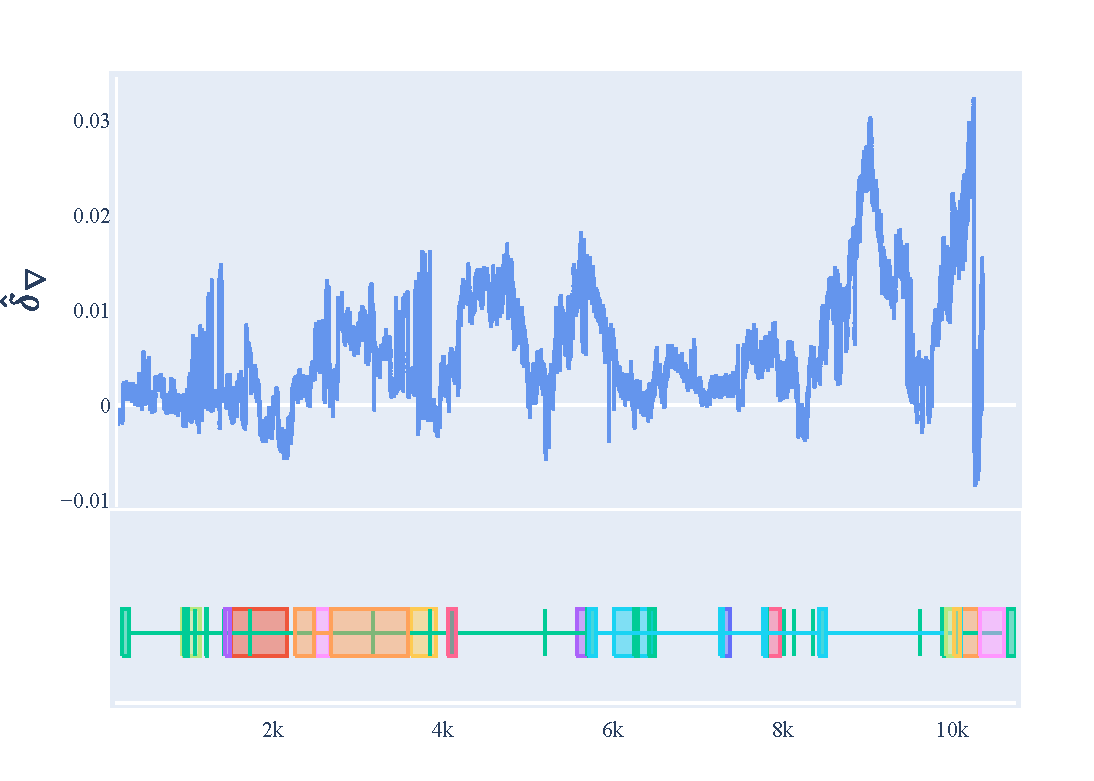
\includegraphics[width=\textwidth]{figures/plots/rodent/dconv-intron3.pdf}
\caption{$\hat\delta_\nabla$.}
\label{fig:rodent/d-conv/intron3}
\end{figure}

The conjectured impact of recombination on the divergence of sequence located within the PAR, is reflected in these developed methods. The results show that although the entire translocated \textit{Fxy} gene rejected the null of mutation equilibrium, the magnitude of disequilibrium was strongest in the half that is now located in the PAR. I uncovered that within the introns there is fascinating pattern of magnitude of disequilibrium, furthermore, the entire pattern is magnified towards the PAR. These results support local rearrangements being a mechanism of mutation disequilibrium and that the more distinct the mutagenic environment in the new location, the higher the magnitude of mutation disequilibrium. Thus, the current understanding of how mutagenesis affects the divergence process is reflected when perturbations happen and there is disequilibrium. Such a positive empirical control adds strength to the confidence in the developed measures and their effective detection and measurements of mutation disequilibrium. 

\section{Testing the unknown}

The question of whether the human genome is at mutation equilibrium is of interest to most humans. Unlike the previous empirical applications, there is no obvious mechanism providing an expectation of the level of mutation disequilibrium. But it is because of the effectiveness of the methods in the previous applications that there are grounds for interpreting the results without such a clear mechanism. I aimed to test for the existence and measure the magnitude of mutation disequilibrium in the human genome. To this end I used intronic and CDS alignments of chromosome 1 of human, chimpanzee and gorilla. Like with previous analyses, the CDS data was alignments of third codon positions only. 

\subsubsection{The majority of the human genome is in mutation disequilibrium}

Q-Q plots of the TOE $\hat p$-value distribution is shown in Figure \ref{fig:primate_lrt_qq}. As with previous analyses, I have included synthetic controls of what the results would look like when the ground truth is that there is no disequilibrium (-ve), and when ground truth is that there is only disequilibrium (+ve). The estimates of the proportion of the analysis that is consistent with the alternate hypothesis, ($1-f$), is $50\%$ for intronic sequence, and $68\%$ for CDS. It is important to note that an assumption of this method of estimation is that data consistent with the null hypothesis is uniformly distributed. 
The -ve control is data generated by the null, for which the data points fall close to the diagonal for intronic data but not so much for CDS, shown in panels a and b of Figure \ref{fig:primate_lrt_qq} respectively. How this small departure from the assumed distributed impacts the methods of estimation is unknown. 

\begin{figure}[h]
\centering
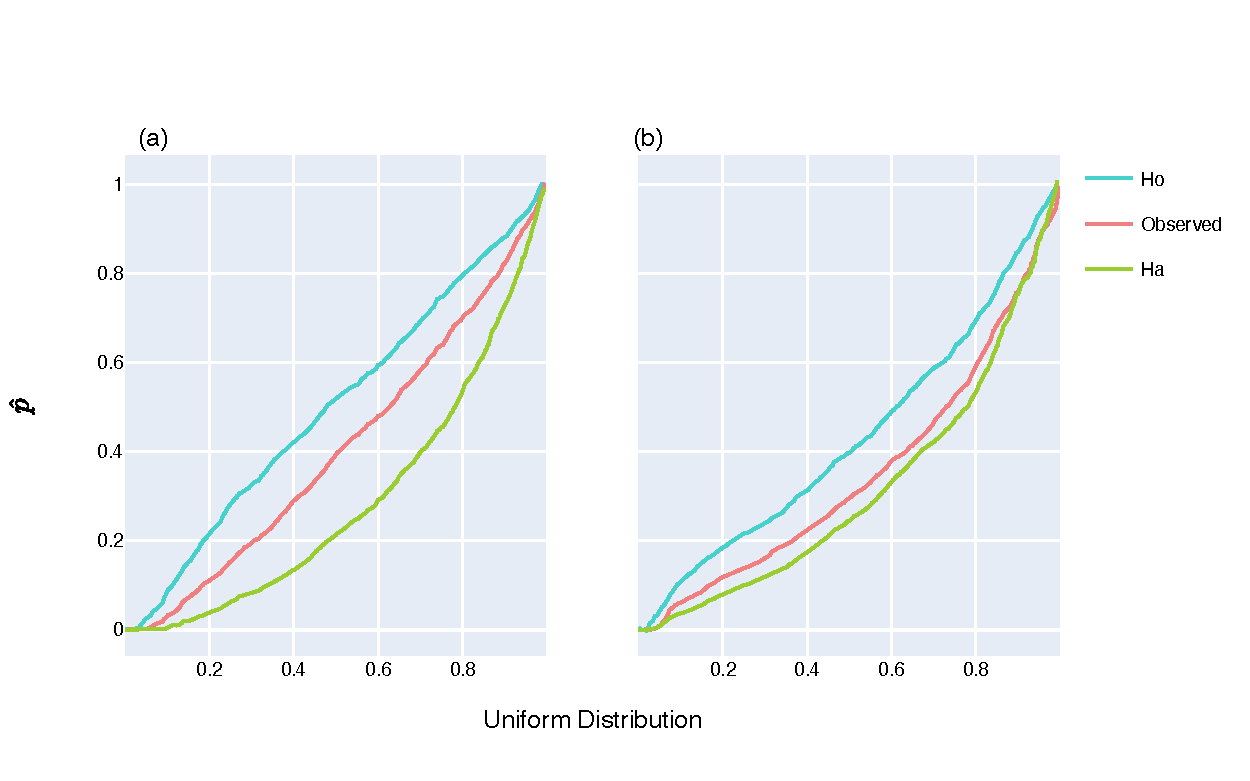
\includegraphics[width=	\textwidth]{figures/plots/primate/LRT-QQ.pdf}
\caption[Humans exhibit a higher proportion of mutation disequilibrium in CDS compared to introns]{\textbf{Humans exhibit a higher proportion of mutation disequilibrium in CDS compared to introns.} The Quantile-Quantile plots compare the distribution of $\hat p-$values to the expected uniform distribution. \textbf{(a)} 1,406 alignments of introns from human, chimpanzee and gorilla, \textbf{(b)}, 1,182 CDS alignments from human, chimpanzee and gorilla. For all model fitting human was the foreground edge. }
\label{fig:primate_lrt_qq}
\end{figure}


\subsubsection{Purifying natural selection impedes the rate of convergence}

On average, the magnitude of mutation disequilibrium is greater in CDS than the corresponding introns. Taking advantage of the paired data structure, I took the difference between $\hat \delta_\nabla$ for the intronic and CDS of the same gene. The resulting distribution, shown in Figure \ref{fig:primate:dconv-diff}, is slightly right shifted, indicating that on average genes have a higher $\hat \delta_\nabla$ in the CDS compared to the intronic sequence. There are, however, a lot of genes for which this is not the case. 

Intronic sequences evolve faster than the exons that encompasses them. A higher level of mutation disequilibrium in the CDS data, when compared to the intronic data, is likely a result of the differing rate of evolution of the two sequence classes. It appeared that owing to a lesser selective constraint, the higher rate of evolution in introns means that sequence of this type was approaching equilibrium faster than the corresponding CDS data. To support the previous result I looked at the branch lengths of the two sequences classes with the expectation that the branch length (measures as the expected number of substitutions) of intronic sequence to be larger than that of the CDS for the same gene. The paired difference in the expected number of substitutions of between introns and CDS is shown in Figure \ref{fig:primate:dconv-diff}. The distribution is shifted to the right, indicating that on average, genes have a higher ENS in the intronic sequence compared to the CDS. 

\begin{figure}[h]
\centering
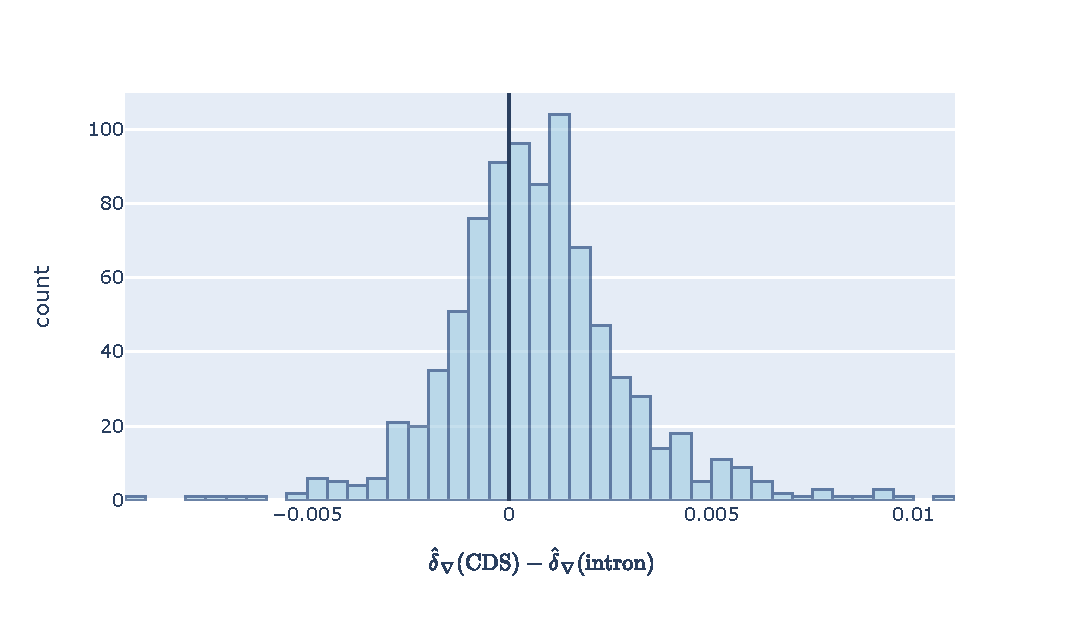
\includegraphics[width=	\textwidth]{figures/plots/primate/d-conv-diff.pdf}
\caption{}
\label{fig:primate:dconv-diff}
\end{figure}


The magnitude of disequilibrium is heterogeneous along a chromosome. Figure \ref{fig:primate:dconv-manhattan} shows $\hat \delta_\nabla$ plotted against the coordinate of the gene on the chromosome for both intronic and CDS. There are clear regions where the average magnitude of disequilibrium is higher than others, this is illustrated best by looking at the first 50M section of introns vs the next 50M section. Interestingly, the overall trend of $\hat \delta_\nabla$ is mirrored between the sequence types. 

\begin{figure}[htbp]
\centering
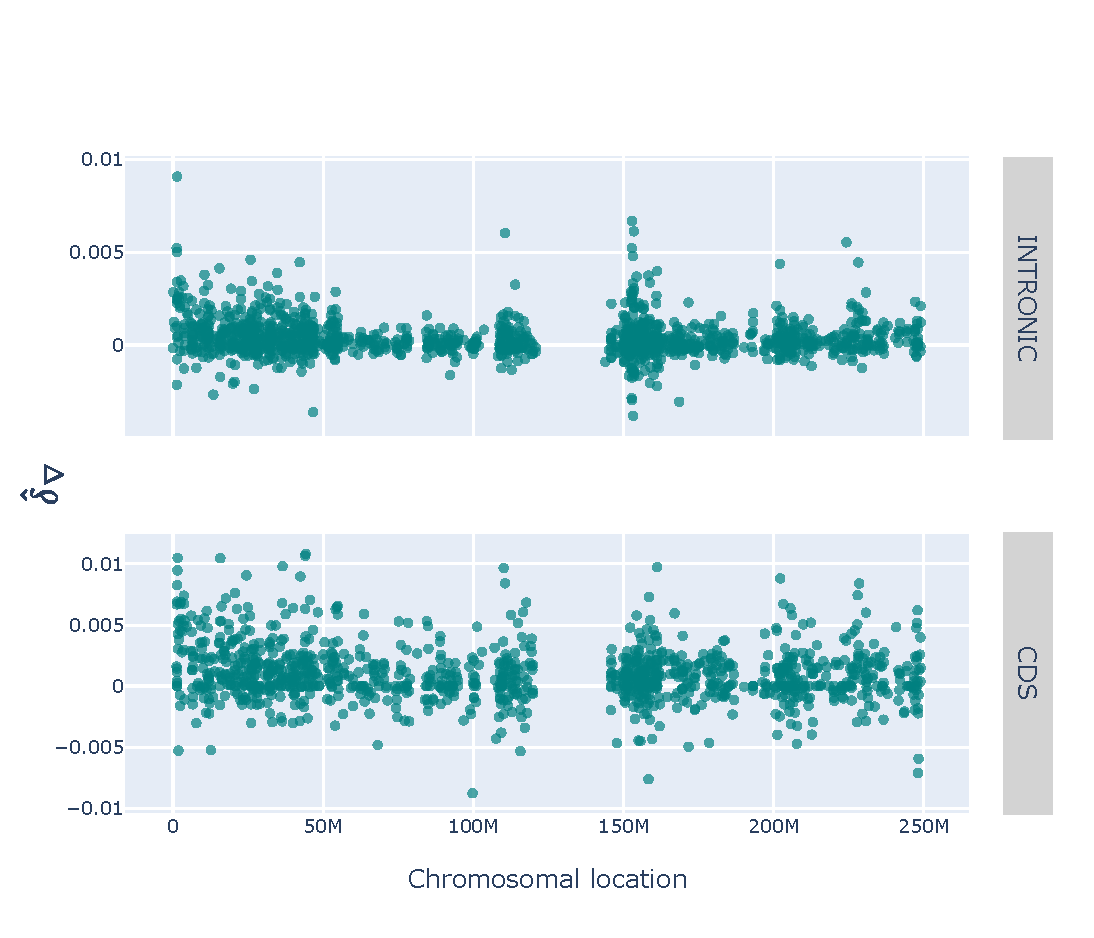
\includegraphics[width=	\textwidth]{figures/plots/primate/d-conv-manhatten.pdf}
\caption{\textbf{The magnitude of disequilibrium is heterogeneous along a chromosome.} Manhattan plots show the position of a gene in a chromosome and the $\hat\delta_\nabla$ for the intronic (top) and CDS sequence (bottom) of that gene. Intronic data included 1,406 alignments CDS data included 1,182. The taxa in all alignments were human, chimpanzee and gorilla, in all model fitting human was the foreground edge. }
\label{fig:primate:dconv-manhattan}
\end{figure}


The results from my analyses show that mutation disequilibrium is pervasive feature of genomes and that the developed methods are effective in robustly detecting and measuring it. In \textit{D. melanogaster}, when DNA methylation with a well-established mutagenic effect is removed, you see a genome-wide increase in disequilibrium. In \textit{M. musculus}, the methods reflect elevated disequilibrium in the region that has moved into the PAR, relative to the component of the gene that remains in the uniquely X region. Applying the methods to Human evolution, I conservatively estimate $>$ 50\% of our genome is in mutation disequilibrium.